\documentclass[10pt]{article}
\usepackage[letterpaper,margin=0.78in]{geometry}
\usepackage[T1]{fontenc}
\usepackage[utf8]{inputenc}
\usepackage{microtype}
\microtypesetup{expansion=false}
\usepackage{amsmath,amssymb}
\usepackage{booktabs,tabularx,array,multirow}
\usepackage{graphicx,xcolor}
\usepackage{caption,subcaption}
\usepackage[numbers,sort&compress]{natbib}
\usepackage[colorlinks=true,allcolors=blue!55!black]{hyperref}
\usepackage{enumitem}
\usepackage{placeins}
\usepackage{titlesec}

\newcommand{\slowlab}{\textsc{SlowLab}}
\newcommand{\Rfinal}{\mathcal{R}_{\mathrm{final}}}
\newcommand{\Rcum}{\mathcal{R}_{\mathrm{cum}}}
\title{\slowlab: Separating Experimental Allocation, Evidence Use, and\\
Recommendation under Slow and Irreversible Feedback}
\author{Anonymous Authors}
\date{}

\begin{document}
\maketitle
\begin{abstract}
Scientific-agent benchmarks rarely test whether an agent can allocate fixed physical
capacity, interpret evidence that arrives during long-running trials, and commit to an
operating recommendation when the experiments themselves incur economic loss. We introduce
\slowlab, a controlled-environment benchmark whose core suite covers interface calibration,
split-plot optimisation, and recommendation after an energy-price shift, with immutable
210-day trials, correlated noise, and separate design-policy and history-reader roles. Exact
hidden-site regret supports model comparisons, while a common-history Bayes-risk diagnostic
asks what an executed design made knowable and how much excess risk remains in the agent's
recommendation. Across 928 frozen model episodes and a separately frozen 384-episode noise
extension, standard design and inference aids do not reliably reduce final regret for the
tested Luna and Sol conditions, and a prespecified half-noise analysis finds a harmful
design-aid effect ($\Delta=0.0113$, 95\% CI $[0.0053,0.0184]$, adjusted $p=0.0096$).
\end{abstract}

\section{Introduction}
\label{sec:intro}

Agents that operate scientific experiments must do more than answer questions about a
finished table. They choose what to run, allocate scarce physical capacity, interpret
partial and noisy evidence, and decide when that evidence supports an operating
recommendation. Existing work evaluates important parts of this loop: BoxingGym limits
sequential experimentation and measures information gain, Olympus and Summit expose
executable optimisation surfaces, Minerva studies noisy parallel batches, and budgeted or
delayed-feedback Bayesian optimisation formalises cost and latency
\citep{boxinggym,olympus,summit,minerva,astudillo2021budgeted,verma2022delayed}. The combined
decision remains difficult to measure when trials occupy a tiered facility, poor experiments
lose real objective value, and a submitted treatment cannot be recalled.

\slowlab{} makes that decision executable in controlled-environment horticulture. A site is
drawn from a documented crop-and-economics distribution. An agent assigns treatments to
named chambers and hydroponic loops, commits them for a 210-day crop cycle, observes only
measurements available by the current simulation time, and recommends an operating point.
Chamber-level climate controls and loop-level cultural controls create a split-plot action
space: replication, treatment coverage, and physical placement compete for the same units.
The published TOMGRO crop model supplies traceability rather than author-independent
difficulty; budgets, ranges, observation channels, and site distributions remain explicit
benchmark choices \citep{jones1999reduced}.

We organise the benchmark around three roles (Figure~\ref{fig:roles}). A \emph{design
policy} chooses treatments and their physical allocation. A \emph{history reader} maps the
time-stamped visible record to a recommendation. A closed-loop agent may implement both in
one model, but fixed-history replay can vary one role while holding the other fixed. The
\emph{evaluator} belongs to the benchmark, may use hidden truth to score the submitted
outputs, and never returns privileged information to the agent.

\begin{figure}[t]
\centering
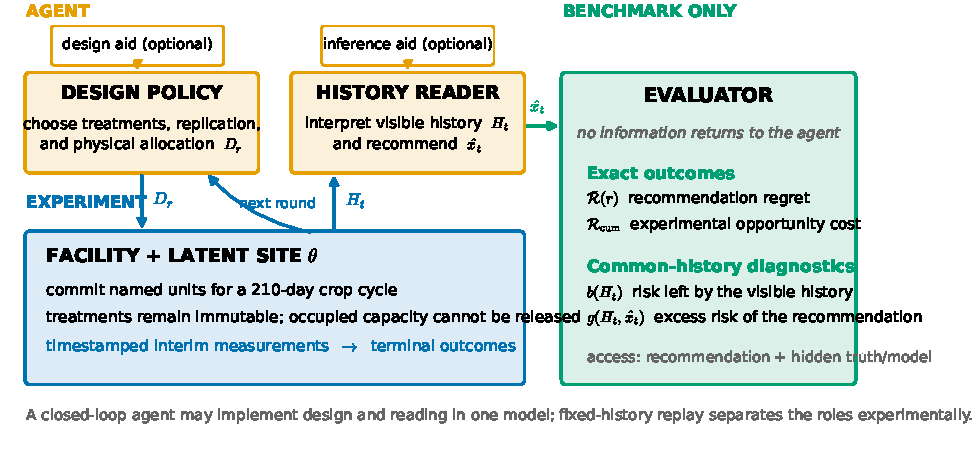
\includegraphics[width=\linewidth]{figures/roles_information_flow.pdf}
\caption{\textbf{Roles and information flow.} The design policy commits treatments and
physical units; the history reader sees only the time-stamped history and produces a
recommendation. The benchmark-side evaluator computes exact outcomes from hidden truth and
calibrated diagnostics from the same visible history. Interim observations may update the
reader and the next design, but cannot alter a committed treatment or release capacity.}
\label{fig:roles}
\end{figure}

Our contribution is threefold. First, we formulate scientific-agent evaluation as coupled
allocation, evidence-use, and recommendation problems under slow, noisy, costly, and
irreversible feedback. Second, we define an information boundary and a common-history
diagnostic that separates what the executed design could support from how the reader used
that evidence. Third, we test scripted policies and model agents in frozen, site-paired
experiments. The resulting claim is deliberately bounded: the tested aids show no reliable
improvement in the primary setting, one lower-noise condition shows harm, and the relative
importance of allocation and reading varies by task.

\section{Decision problem and roles}
\label{sec:framework}

An instance is a latent site $\theta\sim P_\Theta$ defining an objective
$f_\theta:\mathcal X\rightarrow\mathbb R$. In round $r$, the agent observes a timestamped
history $H_r$, chooses a finite design $D_r$, and reports a recommendation $\hat x_r$. A
design contains factor settings and an assignment to available physical units
$\mathcal U_r$; feasibility therefore depends on the facility, not only on whether
$x\in\mathcal X$.

The \emph{design policy} $\pi_D$ maps visible history and remaining resources to a design,
\begin{equation}
 D_r=\pi_D(H_r,\mathcal U_r)\in\mathcal D.
 \label{eq:design}
\end{equation}
It controls what evidence can exist. The \emph{history reader} $\rho$ maps the same visible
history to beliefs and a recommendation,
\begin{equation}
 \hat x_r=\rho(H_r)\in\mathcal X.
 \label{eq:reader}
\end{equation}
Equations~\ref{eq:design} and~\ref{eq:reader} make the separation explicit: the first role controls what evidence can exist, while the second controls how acquired evidence is used. These are analytical roles rather than required software modules; the same LLM produces both outputs in a closed-loop episode.

Submitting $D_r$ occupies its units for a fixed duration $\Delta$. Measurements enter
$H_t$ only when their timestamps are reached. The benchmark permits inspection during a
cycle but does not permit treatment modification, early release, or refunds. Terminal
outcomes follow
\begin{equation}
 y_u=f_\theta(x_u;\phi_u)+\varepsilon_u,
 \qquad \varepsilon\sim\mathcal N(0,\Sigma(D_r)),
 \label{eq:observation}
\end{equation}
Equation~\ref{eq:observation} makes the observation hierarchy explicit: per-unit biological variation $\phi_u$ and chamber, loop, batch, and measurement noise make the covariance structured and treatment dependent. A poor design can therefore fail by
choosing uninformative treatments, confounding them with blocks, or allocating too little
replication.

The \emph{evaluator} is outside the episode policy. It receives designs and recommendations
and may access $\theta$, $f_\theta$, $P_\Theta$, and the forward model. These objects never
enter $H_t$, and evaluator outputs are not fed back to the agent. A design aid may change
$\pi_D$; an inference aid may change $\rho$; neither is an evaluator.

The four regime properties follow directly. Feedback is \emph{slow} because finite
parallel capacity and latency bound evidence per calendar time. It is \emph{noisy} because
one unit does not settle a comparison. It is \emph{costly} because experiments earn the
same economic objective they seek to optimise. It is \emph{irreversible} because committed
capacity and treatments cannot be recovered after later evidence arrives.

\section{Benchmark instantiation}
\label{sec:benchmark}

\subsection{World and facility}
A site seed fixes crop parameters, climate, input prices, and output prices. The forward
model combines reduced TOMGRO physiology with an explicit greenhouse gross-margin model.
Climate chambers are whole plots and independently plumbed hydroponic loops are subplots.
Temperature, photoperiod, lighting, and carbon dioxide are chamber-level controls; density
and pruning are loop-level controls. Observations retain plant, loop, chamber, batch,
measurement, and reporting-resolution variation at their actual scopes.

Each submission names treatments, assigns every treatment to physical units, and supplies a
randomisation seed. Mechanical validation is free and checks capacity, factor bounds, and
control hierarchy. It does not certify statistical quality. Rejected submissions consume no
experimental budget but remain recorded as agent failures.

\subsection{Core tasks}
Table~\ref{tab:tasks} summarises the Version~2 core suite. Its three tasks share the same objective and commitment rule, but differ in the decision being tested rather than serving as nominal difficulty levels.

\begin{table}[t]
\centering\small
\begin{tabular}{@{}lrrrrl@{}}
\toprule
Task & factors & rounds & units/round & unit-days & decision tested \\
\midrule
Sanity   & 1 & 2 & 8  & 3,360  & interface and calibration \\
Optimise & 2 & 3 & 12 & 7,560  & split-plot iteration \\
Transfer & 4 & 3 & 24 & 15,120 & post-shock recommendation \\
\bottomrule
\end{tabular}
\caption{Core Version~2 tasks. Unit-days are committed physical capacity.}
\label{tab:tasks}
\end{table}

\textsc{Sanity} is a one-factor closed-loop and evaluator check. \textsc{Optimise} varies
one chamber-level and one loop-level factor, making allocation and block structure
unavoidable. \textsc{Transfer} varies four resource factors; after the campaign, electricity
and gas prices rise by $2.2\times$ and the agent must recommend again without new trials.

The implementation retains an experimental six-factor \textsc{Screen} configuration, but
we exclude it from the core suite and empirical claims. Its present endpoint is operating
regret, which measures scarce high-dimensional optimisation rather than the stated
screening construct. A valid future version should elicit factor ranks, signs, and
uncertainty and score them directly.

\subsection{Observation timing}
The agent may advance simulation time and request registered modalities from selected units.
Only records whose timestamps have passed are returned. Inspection can update the current
recommendation and, before the next round, its next design. In the synchronous action space
it cannot alter the running treatment, release a unit, or create a replacement batch.

\section{Evaluation}
\label{sec:evaluation}

\subsection{Exact outcome evaluator}
The primary evaluator uses the hidden site only after an action is submitted. Final simple
regret is
\begin{equation}
 \Rfinal(\theta,\hat x)=f_\theta(x^\star_\theta)-f_\theta(\hat x),
 \qquad x^\star_\theta\in\arg\max_{x\in\mathcal X}f_\theta(x).
 \label{eq:final-regret}
\end{equation}
Experimental opportunity cost charges every occupied unit for the objective it forwent,
\begin{equation}
 \Rcum=\Delta\sum_{r=1}^R\sum_{u\in\mathcal U_r}
 \left[f_\theta(x^\star_\theta)-f_\theta(x_u)\right].
 \label{eq:cumulative-regret}
\end{equation}
Equations~\ref{eq:final-regret} and~\ref{eq:cumulative-regret} are exact up to numerical optimisation of the hidden response surface and support the model and tool comparisons. They are reported separately: an agent may find a
good recommendation through an economically poor campaign.

\subsection{Common-history diagnostic}
Outcome regret alone cannot say whether a failure came from missing evidence or poor use of
available evidence. For the history visible at time $t$, define remaining Bayes risk
\begin{equation}
 b(H_t)=\min_{x\in\mathcal X}\mathbb E[\Rfinal(\theta,x)\mid H_t]
 \label{eq:bayes-risk}
\end{equation}
and recommendation excess risk
\begin{equation}
 g(H_t,\hat x_t)=
 \mathbb E[\Rfinal(\theta,\hat x_t)\mid H_t]-b(H_t)\geq0.
 \label{eq:excess-risk}
\end{equation}
In Equations~\ref{eq:bayes-risk} and~\ref{eq:excess-risk}, large $b(H_t)$ indicates that the visible history still leaves a difficult decision, while large $g(H_t,\hat x_t)$ indicates that the recommendation is worse than the best action supported by that same history. Both condition on identical information and therefore avoid the
Version~1 comparison between a preposterior design score and a realised recommendation.

The diagnostic evaluator uses independent posterior samples for action selection and
evaluation. Crop and economic factors update separately until terminal revenue couples
them. We report diagnostics only where calibration error is smaller than the interpreted
effect; all primary claims remain based on exact hidden-site outcomes.

\section{Experimental design}
\label{sec:experiments}

\subsection{Fixed-history role separation}
We first create completed histories using random spread, split-plot DOE, and
constraint-aware batch Bayesian optimisation. Ordinary, block-aware, and component-aware GP
readers receive copies of each accepted history and produce recommendations without changing
any design or observation. Crossing design source with reader makes row differences
allocation effects, column differences evidence-use effects, and residuals interactions.
Privileged readers are labelled as diagnostics and never treated as deployable baselines.

\subsection{Frozen closed-loop study}
The primary matrix runs Luna on \textsc{Optimise} with bare, design-aid, inference-aid, and
combined interfaces: 56 sites, two provider generation seeds per site, and 448 episodes.
Prespecified secondary matrices add a 24-site Sol bare-versus-inference replication, Luna
task heterogeneity on \textsc{Sanity} and \textsc{Transfer}, within-cycle versus
terminal-only access, and a prompt variant, for 928 frozen episodes. A separately frozen
adaptive extension reruns the four Luna interfaces on 16 fresh sites at $0.5\times$,
$1\times$, and $2\times$ observation noise, adding 384 episodes.

Sites are statistical units; provider generations are within-site replicates. We average
generation seeds within site before forming paired differences and use 10,000 site-bootstrap
resamples for percentile 95\% intervals. The primary tool family uses Holm correction;
prespecified secondary families use Benjamini--Hochberg correction. Transport failures may
be retried with the same identity. Format failures, infeasible submissions, and model early
stopping remain outcomes.

\subsection{Post-primary model extension}
A frozen prospective extension compares Luna, DeepSeek V4 Flash 0731, and Qwen 3.8 27B on
the same 24 fresh \textsc{Optimise} sites. Each model runs bare and inference-aid conditions
with two provider generation seeds, for 288 episodes. This extension was specified after the
original Phase~4 analysis and will be reported as post-primary evidence. It estimates three
within-model tool contrasts and same-site pairwise model contrasts; it does not alter the
original primary family.

\section{Results}
\label{sec:results}

\subsection{Allocation and reading are separable and task dependent}
Across held-out fixed histories, the overall range across scripted design sources is
$0.01718$ regret, the range across deployable readers is $0.00619$, and the design--reader
interaction RMS is $0.00209$. This aggregate does not define a universal ordering. The
design range is largest on \textsc{Transfer} ($0.04727$), whereas on \textsc{Sanity} the
reader range exceeds the design range. A block-aware reader also fails to improve over the
ordinary GP on its independent calibration set (paired normalised-regret improvement
$-0.0112$, SE $0.0095$, 24 pairs). Structural readers therefore serve as diagnostics rather than assumed stronger baselines. Table~\ref{tab:phase4-main} places these fixed-history reference points beside the closed-loop results without testing across independently sampled sites.

\begin{table*}[t]
\centering\small
\setlength{\tabcolsep}{4.5pt}
\begin{tabular}{@{}llrrll@{}}
\toprule
Policy & Reader / aid & Sites $\times$ repeats & Mean regret & $\Delta$ vs. bare [95\% CI] & adjusted $p$ \\
\midrule
Random spread & ordinary GP & 8 $\times$ 1 & 0.0072 & descriptive & --- \\
Split-plot DOE & ordinary GP & 8 $\times$ 1 & 0.0128 & descriptive & --- \\
Batch BO & ordinary GP & 8 $\times$ 1 & 0.0066 & descriptive & --- \\
\addlinespace
Luna & none & 56 $\times$ 2 & 0.0128 & reference & --- \\
Luna & design & 56 $\times$ 2 & 0.0129 & +0.0002 [-0.0030, +0.0032] & 1.000 \\
Luna & inference & 56 $\times$ 2 & 0.0108 & -0.0020 [-0.0052, +0.0013] & 0.727 \\
Luna & both & 56 $\times$ 2 & 0.0126 & -0.0002 [-0.0037, +0.0033] & 1.000 \\
\addlinespace
Sol & none & 24 $\times$ 2 & 0.0030 & reference & --- \\
Sol & inference & 24 $\times$ 2 & 0.0035 & +0.0005 [-0.0006, +0.0017] & 0.381 \\
\bottomrule
\end{tabular}
\caption{Final simple regret on \textsc{Optimise} (lower is better). Scripted rows are fixed-history reader replays on eight Phase~3 sites and are descriptive; they are included as reference points, not tested against the independently sampled model runs. Phase~4 model contrasts average two provider generations within each site before inference. Luna tool contrasts use Holm correction across the three preregistered comparisons; the Sol replication uses the prespecified secondary-family adjustment.}
\label{tab:phase4-main}
\end{table*}


\subsection{Standard aids do not reliably reduce final regret}
For Luna on the 56 primary sites, the design-aid difference is $+0.00016$ (95\% CI
$[-0.00299,0.00321]$), inference aid is $-0.00196$ ($[-0.00520,0.00133]$), and both aids
are $-0.00023$ ($[-0.00365,0.00326]$). None is significant after Holm correction. Sol has
lower descriptive regret on its independent sites, but its inference aid also fails to
improve its bare arm: $+0.00053$ ($[-0.00055,0.00173]$), adjusted $p=0.381$. Because the
original Luna and Sol matrices use different sites, their absolute levels are descriptive,
not a paired model ranking.

Table~\ref{tab:phase4-secondary} reports the prespecified secondary and noise-robustness families. The aids were used: inference recommendations were adopted frequently, while geometric design adoption was lower. The null effects therefore do not reduce to complete tool
avoidance. They show that the tested delivery format did not reliably convert adoption into
lower endpoint regret.

\begin{table}[t]
\centering\small
\setlength{\tabcolsep}{4pt}
\begin{tabular}{@{}lrrrl@{}}
\toprule
Contrast & sites & $\Delta$ regret & 95\% CI & adjusted $p$ \\
\midrule
Luna, T1: inference $-$ bare & 24 & -0.0008 & [-0.0053, +0.0037] & 0.722 (BH) \\
Luna, T4: inference $-$ bare & 24 & +0.0114 & [-0.0017, +0.0287] & 0.313 (BH) \\
Luna, within-cycle $-$ terminal-only & 24 & +0.0077 & [-0.0004, +0.0166] & 0.085 (BH) \\
Luna, 0.5$\times$ noise: design $-$ bare & 16 & +0.0113 & [+0.0053, +0.0184] & 0.010 (BH) \\
Luna, 2$\times$ noise: design $-$ bare & 16 & +0.0048 & [-0.0047, +0.0131] & 0.605 (Holm) \\
Luna, 2$\times$ noise: inference $-$ bare & 16 & -0.0067 & [-0.0155, +0.0012] & 0.374 (Holm) \\
Luna, 2$\times$ noise: both $-$ bare & 16 & -0.0040 & [-0.0116, +0.0032] & 0.605 (Holm) \\
\bottomrule
\end{tabular}
\caption{Held-out secondary and robustness contrasts (positive values are worse). The half-noise design-aid contrast is the only listed interval that excludes zero.}
\label{tab:phase4-secondary}
\end{table}


Within-cycle access changes model behaviour and API use, but its paired final-regret
difference is $+0.00768$ (95\% CI $[-0.00041,0.01662]$, adjusted $p=0.085$). Under the
synchronous action space, interim evidence can update a recommendation but has no guaranteed
path to modify running capacity. Testing its operational value requires early termination,
staggered release, or treatment modification.

\subsection{Noise robustness and transfer}
At twice the registered observation noise, all three Luna tool-minus-bare intervals cross
zero. At half noise, the design aid increases regret by $0.01133$ (95\% CI
$[0.00530,0.01842]$, adjusted $p=0.0096$). Other half-noise and one-noise tool contrasts,
and the registered noise interactions, are not significant. The supported conclusion is
therefore bounded: the tested aids show no reliable benefit, and one lower-noise condition
shows harm.

\begin{table}[t]
\centering\small
\begin{tabular}{@{}lrrr@{}}
\toprule
Condition & sites $\times$ repeats & pre-shock & post-shock \\
\midrule
Luna bare & 24 $\times$ 2 & 0.0602 $\pm$ 0.0054 & 0.0681 $\pm$ 0.0095 \\
Luna inference & 24 $\times$ 2 & 0.0716 $\pm$ 0.0074 & 0.1133 $\pm$ 0.0140 \\
\midrule
Inference $-$ bare (post-shock) & 24 sites & \multicolumn{2}{r}{+0.0452 [+0.0200, +0.0781]} \\
\bottomrule
\end{tabular}
\caption{\textsc{Transfer} regret before and after the held-out $2.2\times$ energy-price shock (mean $\pm$ site-level SE). The post-shock paired interval is descriptive because this contrast was not a preregistered inferential family.}
\label{tab:transfer-v2}
\end{table}


Table~\ref{tab:transfer-v2} separates pre-shock and post-shock regret. After the held-out $2.2\times$ energy-price shock, the inference-aid arm has higher regret
than bare by $0.0452$, with a descriptive paired site-bootstrap interval
$[0.0200,0.0781]$. This contrast was not a registered inferential family and motivates a
targeted replication rather than a confirmatory tool claim.

\subsection{Evaluator scope}
On \textsc{Sanity}, independent $32\times32$ crop--economics product posteriors agree to
response-curve RMSE $0.00445$ and select nearly identical Bayes actions. This check does not
establish equal error in higher dimensions. We therefore use exact realised regret for the
claims above and restrict $b(H_t)$ and $g(H_t,\hat x_t)$ to calibrated mechanism analyses.

\section{Related work}
\label{sec:related}

BoxingGym gives agents a finite sequence of experimental queries and evaluates prediction
and expected information gain; it also reports that additional observations do not help
uniformly \citep{boxinggym}. \slowlab{} instead makes physical allocation and experimental
opportunity cost part of the action and separates executed-design support from recommendation
quality. CARE evaluates LLM-guided reaction optimisation under a fixed condition budget;
our emphasis is correlated split-plot allocation and evidence use in a closed-loop physical
campaign \citep{care2026}.

Olympus and Summit provide executable benchmarks for experimental optimisation, while
Minerva adds noisy parallel batches and shared-resource constraints
\citep{olympus,summit,minerva}. These systems motivate realistic surfaces and planners.
\slowlab{} focuses on the information boundary between an agent that operates the campaign
and a benchmark-side evaluator that knows the simulator.

Budgeted Bayesian optimisation studies finite or unknown evaluation costs, and delayed
feedback work studies pending evaluations \citep{astudillo2021budgeted,verma2022delayed}.
Our costs are realised in the objective itself, while tiered controls turn unit assignment
into a split-plot design problem \citep{goos2011splitplot}. The present synchronous action
space exposes within-cycle measurements but does not yet include the staggered replacement
actions needed to realise their full value.

\section{Limitations}
\label{sec:limitations}

The validated domain is simulated greenhouse tomato production. Published physiology and
external price sources improve traceability, but parameter distributions, facility size,
factor ranges, and observation channels remain benchmark choices. Results do not establish
the same tool effects in chemistry, materials, biology, field agriculture, or a physical
greenhouse.

The original frozen model study contains Luna and a smaller Sol replication through one
provider interface. A post-primary same-site Luna--DeepSeek--Qwen extension improves model
coverage but cannot retroactively enlarge the original confirmatory family. Provider routing,
model updates, and prompt format remain sources of external variation.

Within-cycle observation is only consequential through the current recommendation and the
next synchronous design. The environment lacks treatment modification, early stopping,
cleanup cost, residual value, and staggered replacement. It therefore tests whether agents
use interim evidence, not the operational value of adaptive physical intervention.

The common-history evaluator is well calibrated only on the one-factor task. Its finite
candidate search is a lower bound on the world optimum, and its higher-dimensional error is
not fully characterised. Exact hidden-site regret consequently carries the primary claims.

Finally, the experimental \textsc{Screen} configuration does not yet elicit or score factor
selection. Excluding it from the core suite avoids presenting high-dimensional operating
regret as evidence of screening ability; a future task needs direct rank, sign, and
uncertainty targets.

\section{Conclusion}
\label{sec:conclusion}

\slowlab{} evaluates an agent as the operator of a resource-limited experimental campaign.
The design policy determines what evidence can exist, the history reader determines how that
evidence becomes a recommendation, and the evaluator measures both without leaking hidden
truth into the episode. This separation turns a vague failure to ``reason scientifically''
into testable allocation, evidence-use, and recommendation questions.

The current experiments support a narrower conclusion than the Version~1 mechanism story.
Allocation and reading are empirically separable but task dependent. Standard design and
inference aids do not reliably improve endpoint regret in the tested primary conditions; a
fresh high-noise extension preserves that null result, and one lower-noise condition shows
harm. Within-cycle access changes behaviour without improving the final recommendation in
the current synchronous action space. The next decisive tests are matched cross-model
comparisons and action spaces in which interim evidence can change physical capacity.

\bibliographystyle{plainnat}
\bibliography{refs}
\appendix
\section{Protocol and reproducibility}
\label{app:protocol}

The frozen experiment families are:
\begin{itemize}[leftmargin=1.3em,itemsep=0.2em]
\item Primary: \nolinkurl{slowlab-v2-phase4-confirmatory-2026-09-13-a2}, with 928 complete and unique expected episode identities.
\item Noise extension: \nolinkurl{slowlab-v2-phase4-noise-robustness-2026-09-19-a2}, with 384 complete rows.
\item Post-primary model extension: \nolinkurl{slowlab-v2-phase5-model-extension-2026-09-20-a1}.
\end{itemize}
Each record stores requested and actual model identifiers, provider, generation seed, prompt
hashes, usage, cost, retry attempt, finish reason, format failures, infeasible submissions,
and the accepted event history.

The public numerical source for the current tables is
\nolinkurl{results/phase5_paper_summary_env2.0.0.json}. From an unpacked frozen data bundle,
\nolinkurl{scripts/reproduce_phase5_paper.py} rebuilds analyses, generated tables, figures,
claim checks, cross-reference checks, and the PDF. Private review notes are excluded from
the repository artifact.

\section{Reference policies}
Random spread maximises geometric coverage subject to the same facility validator as model
agents. Split-plot DOE balances whole-plot combinations across chambers and randomises
loop-level settings within chamber. Constraint-aware batch Bayesian optimisation fits an
ordinary GP to completed outcomes and proposes a feasible batch by sequential
fantasisation. Reader replay copies each accepted completed history to ordinary,
block-aware, and component-aware GPs without changing a design or observation.

\section{Deferred dynamic actions}
The current environment records time-stamped interim measurements but exposes no treatment
change, early termination, cleanup, residual-value, or asynchronous replacement action.
Adding one requires explicit transition dynamics and a matched oracle. Until then, claims
about the value of within-cycle observation are restricted to recommendation and next-round
behaviour.

\end{document}
